%' Directed acyclic graph (DAG) with arrow text annotations
%'
%' @src: Figure 6 in Theory-Driven Analysis of Intra-individual Dynamics 
%' @url: https://yongfu.name/intra/main.pdf

% \documentclass[12pt,preview,border=0]{standalone}
\documentclass[border=0]{article}
\usepackage[paperheight=10cm,paperwidth=10cm]{geometry}
\usepackage{graphicx}
\usepackage{amsmath}
% \usepackage{kmath,kerkis}
\usepackage{tikz}
\usetikzlibrary{arrows,automata,positioning}

\begin{document} 
\thispagestyle{empty}% Reset page style to 'empty'

\begin{center}
Dawid-Skene Model \\

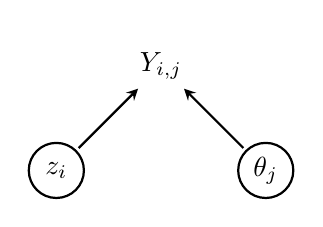
\begin{tikzpicture}[
	> = stealth, % arrow head style
	shorten > = 1pt, % don't touch arrow head to node
	auto,
	node distance = 2cm, % distance between nodes
	thick, % line style
	U/.style={circle, draw=black, inner sep=0.5pt, outer sep=1.5pt, minimum size=7mm, font=\normalsize},  %draw=black, fill=white
	O/.style={circle, inner sep=3.4pt, outer sep=-3pt, minimum size=7mm, font=\normalsize},              %draw=white, fill=white
	]
	
	% Nodes and their relative positions
	\node[O] (Y) {$Y_{i,j}$};
	\node[U] (Z) [below left  = 1.1 of Y] {$z_i$};
	\node[U] (T) [below right = 1.1 of Y] {$\theta_j$};

	% Paths connecting nodes
    \path[->] (Z) edge (Y);
	\path[->] (T) edge (Y);

\end{tikzpicture}

\newpage
\thispagestyle{empty}% Reset page style to 'empty'


Item Response Theory \\

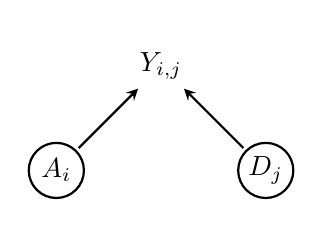
\begin{tikzpicture}[
	> = stealth, % arrow head style
	shorten > = 1pt, % don't touch arrow head to node
	auto,
	node distance = 2cm, % distance between nodes
	thick, % line style
	U/.style={circle, draw=black, inner sep=0.5pt, outer sep=1.5pt, minimum size=7mm, font=\normalsize},  %draw=black, fill=white
	O/.style={circle, inner sep=3.4pt, outer sep=-3pt, minimum size=7mm, font=\normalsize},              %draw=white, fill=white
	]
	
	% Nodes and their relative positions
	\node[O] (Y) {$Y_{i,j}$};
	\node[U] (Z) [below left  = 1.1 of Y] {$A_i$};
	\node[U] (T) [below right = 1.1 of Y] {$D_j$};

	% Paths connecting nodes
    \path[->] (Z) edge (Y);
	\path[->] (T) edge (Y);

\end{tikzpicture}
	

\end{center}\end{document}
